\documentclass[12pt, twoside]{article}
\usepackage[letterpaper, margin=1in, headsep=0.5in]{geometry}
\usepackage[english]{babel}
\usepackage[utf8]{inputenc}
\usepackage{amsmath}
\usepackage{amsfonts}
\usepackage{amssymb}
\usepackage{tikz}
\usepackage{yhmath}
%\usetikzlibrary{quotes, angles}

\usepackage{graphicx}
\usepackage{enumitem}
\usepackage{multicol}

\usepackage{fancyhdr}
\pagestyle{fancy}
\fancyhf{}
\renewcommand{\headrulewidth}{0pt} % disable the underline of the header

\fancyhead[RE]{\thepage}
\fancyhead[RO]{\thepage \\ Name: \hspace{3cm}}
\fancyhead[L]{BECA / Dr. Huson / 10th Grade Geometry\\* 10 June 2019}

\begin{document}
\subsubsection*{13.7 Homework: Cross sections, distance applications}
 \begin{enumerate}

   \item In the diagram below, $\triangle ABC$ has vertices with coordinates $A(1,3)$, $B(6,3)$ and $C(4, 7)$.
     \begin{center} %4 quadrant regents grid
       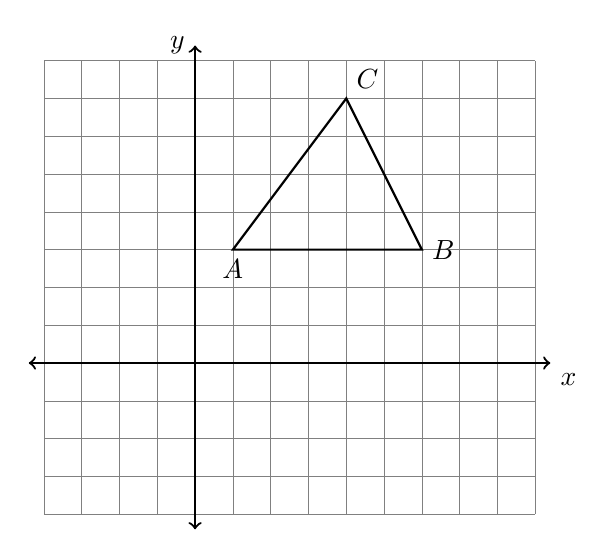
\begin{tikzpicture}[scale=.48]
         \draw [help lines] (-4,-4) grid (9,8);
         \draw [thick, <->] (-4.4,0) -- (9.4,0) node [below right] {$x$};
         \draw [thick, <->] (0,-4.4)--(0,8.4) node [left] {$y$};
         \draw [thick]
           (1,3)node[below]{$A$}--
           (6,3) node[right]{$B$}--
           (4,7) node[above right]{$C$}--cycle;
         %\draw [fill] (-1,2) circle [radius=0.1] node[above left] {$A$};
         %draw [fill] (8, -4) circle [radius=0.1] node[below right] {$C$};
       \end{tikzpicture}
     \end{center}
     Find the length of each side of $\triangle ABC$, showing that it is isosceles and not equilateral.\\[0.5cm]
     \begin{tabular}{c|c|c}
       $AC=$ & $BC=$ & $AB=$ \\
       $\sqrt{(x_C-x_A)^2+(y_C-y_A)^2}$ & $\sqrt{(x_C-x_B)^2+(y_C-y_B)^2}$ & $ \sqrt{(x_B-x_A)^2+(y_B-y_A)^2}$ \\
       & & \\
       & & \\
     \end{tabular} \vspace{6cm}


   \item Find the length of the line segment $A(1,3)$ $B(3,7)$. Simplify the radical.

\newpage

  \item On the set of axes below, graph the quadrilateral $ABCD$ having coordinates $A(-3,-3)$, $B(5,1)$, $C(6,8)$, and $D(-2,4)$.
    \begin{center} %4 quadrant regents grid
    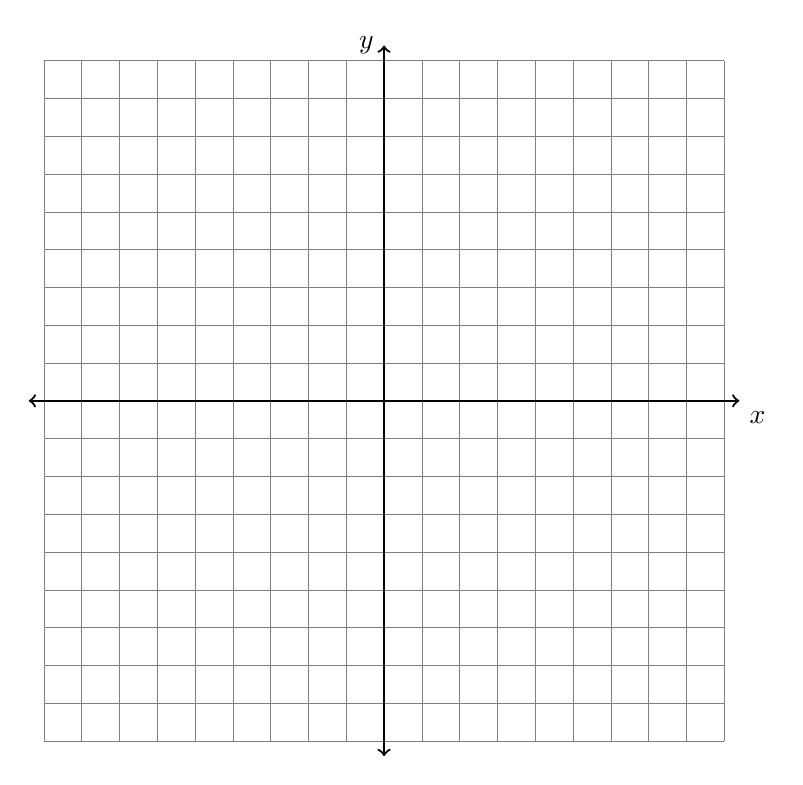
\begin{tikzpicture}[scale=.48]
      \draw [help lines] (-9,-9) grid (9,9);
      \draw [thick, <->] (-9.4,0) -- (9.4,0) node [below right] {$x$};
      \draw [thick, <->] (0,-9.4)--(0,9.4) node [left] {$y$};
      %\draw [thick] (-3,-3) node[below] {$A$}--
      %(5,1) node[right] {$B$}--
      %(6,8) node[left] {$C$}--
      %(-2,4) node[left] {$D$}--cycle;
      %\draw [fill] (5,0) circle [radius=0.1] node[above left] {$P$};
    \end{tikzpicture}
    \end{center}
    Find the length of each side of the quadrilateral.

\newpage
  \item A staircase riser is cut as a series of congruent triangles with each step's ``rise" equal to 8 inches, and the ``run" of each step is 10 inches, as shown below. ($AB=8$ and $BC=10$) Find the diagonal length of the two-step riser, the distance $AE$, to the \emph{nearest inch}.\\[0.5cm]
       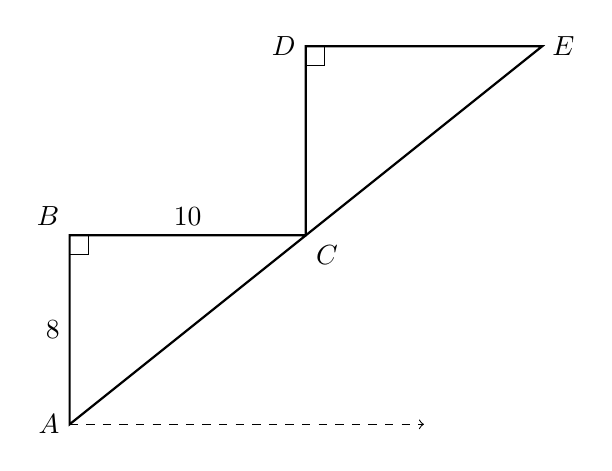
\begin{tikzpicture}[scale=0.3]
         \draw [thick]
         (0,0)node[left]{$A$}--
         (0,8)node[above left]{$B$}--
         (10,8)node[below right]{$C$}--
         (10,16)node[left]{$D$}--
         (20,16)node[right]{$E$}--cycle;
         \draw [dashed, ->] (0,0)--(15,0);
         \draw (0,8)++(0,-0.8)--++(0.8,0)--+(0,0.8);
         \draw (10,16)++(0,-0.8)--++(0.8,0)--+(0,0.8);
         \node at (0,4)[left]{$8$};
         \node at (5,8)[above]{$10$};
         %\node at (28:1.5)[right]{$x$};
       \end{tikzpicture}


   \item As shown in the diagram below, the radius of a cone is 2.5 cm and its slant height is 6.5 cm.\\[0.5cm]
     \includegraphics[width=0.25\textwidth]{cone_Jan2019-23.png}
     \begin{enumerate}
       \item Find the height of the cone. \vspace{2cm}
       \item How many cubic centimeters are in the volume of the cone? Express your answer in terms of $\pi$.
   \end{enumerate} \vspace{2.5cm}

\newpage
  \item Which three-dimensional figure will result when a rectangle 6 inches long and 5 inches wide is continuously rotated about the longer side?
    \begin{enumerate}
      \item a rectangular prism with a length of 6 inches, width of 6 inches, and height of 5 inches
      \item a rectangular prism with a length of 6 inches, width of 5 inches, and height of 5 inches
      \item a cylinder with a radius of 5 inches and a height of 6 inches
      \item a cylinder with a radius of 6 inches and a height of 5 inches
    \end{enumerate}

  \item An isosceles right triangle whose legs measure 6 is continuously rotated about one of its legs to form a three-dimensional object. The three-dimensional object is a
    \begin{enumerate}
      \item cylinder with a diameter of 6
      \item cylinder with a diameter of 12
      \item cone with a diameter of 6
      \item cone with a diameter of 12
    \end{enumerate}

  \item A right cylinder is cut perpendicular to its base. The shape of the cross section is a
    \begin{enumerate}
      \item circle
      \item cylinder
      \item rectangle
      \item triangular prism
    \end{enumerate}

    \item Simplify each expression. (Leave it in radical form if necessary, not a decimal.)
      \begin{enumerate}
        \begin{multicols}{2}
        \item   $\sqrt{121}$ \vspace{1.25cm}
        \item   $\sqrt{48}$
        \item   $\sqrt{27}$ \vspace{1.25cm}
        \item   $\sqrt{8}$
        \end{multicols}
      \end{enumerate}



\end{enumerate}
\end{document}
